% this is a template for an ``article'' document, the most common
% for research papers. Theses may be better written in the ``report''
% format.

\documentclass{article}
\usepackage{graphicx} 
\usepackage{amsmath}
\usepackage{paralist}
\usepackage{wrapfig}
\usepackage[all]{xy}
\usepackage{cite}


% set margins to 1 inch all around the page, no header or footer.
\setlength{\textheight}{9in}
\setlength{\textwidth}{6.5in}
\setlength{\topmargin}{-0.125in}
\setlength{\oddsidemargin}{-.2in}
\setlength{\evensidemargin}{-.2in}
\setlength{\headsep}{0in}

% enable insertion of graphics, ``smart'' line spacing, long tables
% for the long (i.e. more than 1 page) tables, refer to supertab.ps
\usepackage{setspace,supertabular}	

%\usepackage[dvips]{graphicx}
% use \usepackage[dvips,draft]{graphicx} during document creation if
% you have screenshots in your file.


% output the list of used files to the terminal during compilation.
% this helps to keep track of the figures and tex-files you are using.
\listfiles

% set the path for figures.
% all figures should be in a subdirectory under the document directory
\graphicspath{{figures/}}

% define the line spacing. Footnotes and Caption remain single-spaced
\singlespacing
% alternatives: \onehalfspacing or \doublespacing or \setstretch{1.6}


% this was the preamble, now comes the main text
\begin{document}

\section{Robust Dynamic Programming}
Model based optimal control is a powerful tool but relies heavily on the accuracy of the system model, which is not a trivial task to derive. There are many parameters involved, such as friction, sensor readings, calibrations, and the model may change over time due to wear, temperature, humidity, contact condition, and others.

Eric Whitman looks into using Multiple Model Dynamic (MMD) Programming, and uses the inverted pendulum swing-up problem to demonstrate the algorithm. \cite{eric_thesis}
 
By using the content provided in his thesis, the references, and example code, work on providing other students comprehensive guild on MMD for future students, we are looking at the different advantages, and shortcomings that comes with the algorithm.

Based on his previous work this paper aims to clarify the fundamental concepts of MMD and provide graspable examples. Furthermore, a faster running-time implementation using a General Purpose Graphical Processing Unit (GPGPU).

\subsection{Looking at a Problem}
To have a better understanding on how the algorithm works, we are going to look at the  inverse pendulum swing-up example, which consists of a motor attached to the end of pendulum, and the controller aims to bring the pendulum to an upright position by applying torques based on the current state of the system. 

The expected behavior for the control law is to apply a torque equal to the direction the pendulum is swinging, such that more energy is added to the pendulum with each period, and when the pendulum finally has enough energy to perform a full rotation, apply a torque opposite to the movement such that the pendulum stops in an upright position.  

Since our interested is in solving a variety of dynamic programming problems, we are going to look at a more generic solution that discretizes the whole state of problem, and attempts to find a adequate policy to reach the desired goal.

We are going to assume that the pendulum has a length, $L=1m$, and a weight, $m=1kg$, and the world has a gravity $g=9.81\frac{m}{s^2}$. The pendulum has a 2-dimensional state space, $\theta$, the angle of the pendulum relative to the up position, and $\omega$, the current velocity in radians per second. There is only a one-dimension action space, $\tau$, the force of the motor can apply, and limit it at $\pm 1.5 \frac{N}{s}$.

The pendulum dynamics can be described by:

\begin{equation} 
\dot{\omega} = \frac{mLg \cdot sin(\theta) + \tau}{mL^2}
\end{equation}

Define the state space as $x=\{\theta, \omega\}$, and the action space to be $u=\{\tau\}$. We define the pendulum to be pointing up at, $\theta = 0$, and we are optimizing the pendulum to reach $\theta = 0$, with zero velocity, $\omega = 0$, using the minimum torque necessary. We define the cost function be to $L$:

\begin{equation} 
L(x,u) = \theta^2 + 0.5 \cdot \omega^2 + \tau^2
\end{equation}

And we want to minimize the total cost function, C, given by the integral: 

\begin{equation} 
C = \int L(x,u) dt
\end{equation}

We discritize the state space of the pendulum by assuming $\theta \in  (-\pi,\pi)$, and $\omega \in (-10,10)$, and define a 2-dimensional increments of 0.016 radians, and 0.022 radians/second, giving us a table of 360,000 states. We also assume a time step of T=0.003 second delay between each action, and sensor reading of the current pendulum state. We define the iteration function:

\begin{equation} 
x_{k+1}(u) = 
\begin{bmatrix}
\theta_{k+1} \\
\omega_{k+1}
\end{bmatrix}
=
\begin{bmatrix}
\theta_{k} + T \cdot \omega_{k} + \dot{\omega} \cdot T^2 \\
\omega_{k+1}
\end{bmatrix}
\end{equation}

For each state of the pendulum, we define two elements, the value $V(x) = {v}$, and let the initial value of $V(x)=0$ for all $x$, and the policy $U(x)={\tau}$, and let the initial value for all states be equal to 0. For optimizing the policy, we guess a random torque, $\tau'$, for every state in the grid, x, and define:

\begin{equation} 
V'(x) = C(x,u) + \gamma V(x_{k+1}(\{\tau '\}))
\end{equation}

And if $V'(x)<C(x,u) + \gamma V(x_{k+1}(U(x)))$, we let $V'(x)$ and $U(x)={\tau'}$.

We run the previous operation on all states of the grid for an uncertain number of times. For this particular program, running this optimization for 1000 iterations is siffucient for making the pendulum converge to the desired goal state, but it can also be noted that running for 10000 times generates a more torque efficient solution.

The problem is simple enough with the single-link pendulum case, but when extra links are added to the pendulum, such as the double-link pendulum, the problem becomes increasingly difficult to solve, but the algorithm can still find a sub-optimal policy with the modifications of redefining the state space, action space, and the iterate function.

\subsection{Running through an example}

To better comprehend how this problem is solved, let’s take a first iteration from a single discrete point in the grid. Suppose we are analyzing the $\omega_0=\frac{\pi}{2}, \omega_0=1 rad/sec$, and since we are in the first iteration, our current policy is $\tau_0=0$. If we keep the current torque, we find that the next step is:
	
\begin{equation} 
\dot{\omega_0} = \frac{1 \cdot 1 \cdot 9.81 \cdot sin(\frac{\pi}{2})+0}{1 \cdot 1^2} = 9.81
\end{equation}

\begin{equation} 
\begin{bmatrix}
\theta_{k+1} \\
\omega_{k+1}
\end{bmatrix}
=
\begin{bmatrix}
\theta_{k} + T \cdot \omega_{k} + \dot{\omega} \cdot T^2 \\
\omega_{k+1}
\end{bmatrix}
=
\begin{bmatrix}
\frac{\pi}{2}+1 \cdot 0.003 + 0.5 \cdot 9.81 \cdot 0.0032 \\
1 + 9.81 \cdot 0.003
\end{bmatrix}
=
\begin{bmatrix}
\frac{\pi}{2}+0.003044145 \\
1.02943
\end{bmatrix}
\end{equation}

And we can now discover the current value of $V(x)$ to be:
\begin{equation} 
V(x) = C(x,u) + \omega V(x_{k+1}(\{\tau'\})=(\theta^2+0.5 \cdot \omega^2 + \tau^2)+1 \cdot 0 = 2.6032705
\end{equation}

Since this is the first iteration of this equation, the second term of the value equation is 0. Now suppose that we guess $\tau=1$, and find the new state to be:


\begin{equation} 
{x'}_1 = 
\begin{bmatrix}
\frac{\pi}{2} + 0.003048645 \\
1.03243
\end{bmatrix}
\end{equation}

We find the new value of
\begin{equation} 
V'(x) = 2.6062750
\end{equation}

Since $2.6032705 < 2.6062750$, we learn that we are applying a torque in the wrong direction, and it is better to let gravity pull on the pendulum instead of applying addition torque, and keep the value, $U(x)={0}$. Now suppose we guess $\tau = -1$, we find that 
\begin{equation} 
{x'}_1 = 
\begin{bmatrix}
\frac{\pi}{2} + 0.003039645 \\
1.02643
\end{bmatrix}
\end{equation}
With the value
\begin{equation} 
V'(x) = 2.6002660
\end{equation}

Since $2.6032705 > 2.6002660$, we change the value $U(x_0)={-1}$. Giving a new optimal torque to apply at that point.

It is important to notice the optimal torque may completely change directions throughout the iterations due to the value of the neighbours changing. (Further details with the video)

\subsection{Analysing this solution}
The algorithm is far from being real time, since for the single-link pendulum case, on an 8-core CPU at 2.8GHz, takes about 4 seconds for each iteration, and about 1 hour for the 1000 iterations, but it does generate very robust policy tables.

On the following plot we show the policy of 10,000 iterations running against a pendulum, position of the pendulum relative to the up position, starting at pi, pointing down, and with 0 velocity. It is interesting to see that the policy follows similar to a bang-bang controller, using near maximum torque on both directions, until the system has enough energy to reach the necessary solution. (TODO: Talk about behavior near t=45seconds, where the exact amount of force is applied to get the up position)

\subsection{CUDA}

To first understand why using a GPGPU is a faster tool that fits to solve this problem, we must first take a look at the history of how games and GPUs, and how the computing model of GPU’s fits this problem.

The principles of a modern game rendering have not changed much since the beginning; A list of triangles in 3d space are transformed, projected into a plane, and then each pixel is rendered with the color of the closest triangle. The three major steps in the rendering pipeline involves:

\begin{enumerate}
\item Vertex processing: Each vertex in a model is moved into a new position by transformation matrices and weights.
\item Rasterization: Processing each of the triangles in the screen region, and calculating what the closest triangle in each pixel is.
\item Fragment shading: Determined the color of each pixel based on the closest triangle. (The coordinates of the closest triangle is passed into the fragment shader)
\end{enumerate}

While the second step is usually done by hardware, hidden away from developers, the main aspects of the first and third step is that each vertex and pixel can be completely independent of one another and can be programmed by C-like programs, called shaders. Due the popularity and profitability

of game companies, this gave incentives for companies to develop dedicated hardware that process each of the points as quickly as possible.

Until 2001 developers could only use shaders that were pre-programmed into the hardware, and then Direct3D 8 \cite{wiki:direct3d} gave developers the option to program custom shaders that run in the hardware.

The main drive for GPU development was for computer graphics, but using some technique, one could speed up large linear algebra processing using storage through image textures. \cite{Goeddeke:2005:GBM}

For example, OpenGL could be used to perform the multiplication of two 256 by 256 matrices. In this case, three texture buffers would be created inside of the GPU, each of the size of the matrix, and two of them would be loaded with the read-only input matrices values from the main computer memory, while the other one would be used as a render texture. When the fragment shader runs over all the pixels of the render texture, the user defined program would read the necessary values from the other two matrices and render the corresponding output value. 

Later during 2007, NVIDIA released CUDA, a general purpose computing standard that would allow developers to create GPU based software, and later on 2008, the open source community followed with OpenCL. While OpenCL and CUDA follows the same principles as fragment shaders, it also opened doors for other applications, such as atomic operations, thread syncing, memory barriers, and others.

\pagebreak

\section{DARPA Robotics Challenge}
\paragraph{The objective of this paper is to help the reader understand the current workings of the Carnegie Mellon’s University’s controller.}  
 
The DARPA Robotics Challenge (DRC) is a competition of teams developing robots capable of assisting humans in responding to natural and man-made disasters.   
 
Teams are spread in several tracks. WPI is in the Track C team, in which competed in the Virtual Challenge (DVC), and received funding for the Atlas robot.  

\section{Hardware}
\subsection{Atlas}

The Atlas robot is a powerful robot in the form of an adult human. It is powered by 28 hydraulically-actuated rotation joints, with a closed-loop position and force control. It also contains a real time control computer (What is the specs?). Currently powered by external electricity, and packed with a head-mounted sensor package with LIDAR and stereo cameras. 

\subsection{DBI Behaviors}
Boston Dynamics provided predefined behaviour for Atlas, each of these controllers can be activated from state to another state. 

\subsubsection{Manipulate}
\begin{wrapfigure}{r}{0.3\textwidth}
  \begin{center}
    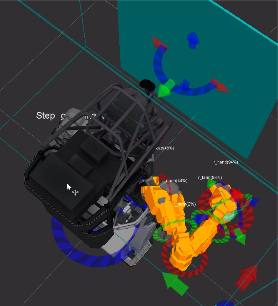
\includegraphics[scale=0.5]{images/align_to_wall.png}
  \end{center}
  \caption{Rviz within ROS}
\end{wrapfigure}
The Manipulation mode, in which the user can control all the joints above the torso, and basic control of the pelvis orientation, and the pelvis height. The legs are controlled by the Boston Dynamics controller embedded in the firmware.

It is fairly easy to use, and has a wide range of motion if the pelvis position and orientation is controlled together with an inverse kinematics solver for the joints, but can be unpredictable. The robot has the problem that the back joint that helps torso move back and forth is not strong enough to hold, and may give out a times, causing the whole top part of the robot fall forward, or at times, make the entire robot fall forward. 

The user has the option to input any additional weight that the hand is carrying to help the controller.

MoveIt! is a software developed with ROS to help robot developers control the robot. It contains a inverse kinematics solver that can interface with Atlas, but prevents two containing limitations: 
\begin{inparaenum}[\itshape a\upshape)]
\item The inverse kinematics solver has no option to give approximate solutions, and will fail to give joint state values unless a very approximate solution for a desired hand position exists.
\item It does not account for modifying the pelvis position and orientation for solving for a solution. \end{inparaenum}
 
\subsubsection{Walk}

\begin{wrapfigure}{r}{0.3\textwidth}
  \begin{center}
    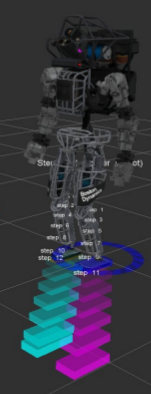
\includegraphics[scale=0.5]{images/step_gui.png}
  \end{center}
  \caption{The planned steps for the robot walking forward and to the left}
\end{wrapfigure}


Boston Dynamics walking behaviour works by the user providing a sequence of steps paramters, which include the step duration, sway duration, swing height, lift height, and step end distance.  

The WPI team developed an additional interface for Rviz, such as the robot driver is able to specify a final desired feet positions for the robot, and the software produces all the intermediate steps. It took some trial-and-error testing to figure out what the maximum step size are possible, and the program does not account for any debris on the floor. 

Although it could be automated, it is also usually required for the driver to additionally modify the final two steps such that they are further apart, thus providing a stronger base for the walking. 

\subsubsection{Atlas Control Parameters}
There exists several controller parameters that is hidden to the developer that controls the hydraulic joints. We let $q$, $qd$ and $f$ be the senses position, velocity, and torque respectively. And we let $q_d$, $qd_d$, and $f_d$ be the desired position, velocity, and torque for each joint.

We create the following variables to help control the desired torque control:

\begin{itemize}
\item $k_{q_p}$: Position error gain, in $\frac{N \cdot m}{rad}$.
\item $k_{q_i} $: Integral of position error gain, in $\frac{N \cdot m}{rad \cdot s}$.
\item $k_{{qd}_p}$: Derivative error gain, in $\frac{N \cdot m}{\frac{rad}{s}}$.
\item $k_{f_p}$: Proportional force feedback gain.
\item ${ff}_{qd}$: Feedforward velocity gain.
\item ${ff}_{{qd}_d}$: Feedforward desired velocity gain.
\item ${ff}_{f_d}$: Feedforward desired force gain.
\item ${ff}_{const}$: Constant force term.
\end{itemize}

And use them accordingly: 
\begin{align*}
k_{q_p} &\cdot ( q_d - q ) &+\\
k_{q_i} &\cdot 1/s * ( q_d - q ) &+\\
k_{{qd}_p} &\cdot ( {qd}_d - qd ) &+\\
k_{f_p} &\cdot ( f_d - f ) &+\\
{ff}_{qd} &\cdot qd &+\\
{ff}_{{qd}_d} &\cdot qd_d &+\\
{ff}_{f_d} &\cdot f_d &+ {ff}_{const}
\end{align*}


\subsection{Robotiq Hand}

The robot gives the option of interchanging the hands, the two primary options being the iRobot© hands, and the Sandia© hands. While both options are known companies in the industry, neither provided the power, nor robustness necessary to complete the industrial tasks. These hands were designed to perform precision tasks, such as picking up a coin, or a fist-sized rock, but not to pick up a power tool. The team went to an alternative in using hardware developed Robotiq©, a 3-Finger adaptive robot gripper, which provided a much stronger grip. 



\section{Software}
The software developed my WPI and CMU are mostly written in C++, with small parts written in Python. 

\subsection{Architecture}

The controller has three main aspects: 

\subsubsection{Motion controller}
The motion controller is responsible for controlling the joints of the robot. 

Most of the math executed is done with the help with Eigen, a C++ template library for linear algebra. 


\subsubsection{Vision}

\subsubsection{High-level controller}


\subsection{Network}
\subsection{ROS}

\section{Full-body controller}
Intro...Carnegie Mellon University developed custom software for controlling the robot, which involves two major aspects that are solve using Quadratic programming, an Inverse Kinematics solver, and an Inverse Dynamics solver. 

\subsection{Inverse Kinematics}
Inverse kinematics is the process of given an desired end effector position, generate a joint state that will as close as possible achieve the goal. There exists a great deal of research, and libraries that provide fast and concise solutions, but most of the research assumes that the base of the joint system does not move, such as one that you might find on a factory. 

Atlas is a bipedal robot, it is not simple to define a set of rules that describes all possible motions. 

The library SD/Fast provides physically-based simulation of mechanical systems by taking a short description of an articulated system of rigid bodies and deriving the full nonlinear equations of the system. \cite{sdfast} The library takes several key factors about each sub-body in the robot, such as the link positions, mass, and inertia. The library than generates a C file that provides informations such as the center of mass, jacobians, and positions. 

During this current iteration we have the following competing Jacobians that control the robot: 
\begin{enumerate}
\item Left/Right hand position: Global desired Cartesian coordinates.
\item Left/Right hand orientation: Three local desired euler angles.
\item Torso orientation: Three local desired euler angles.
\item Pelvis orientation: Three local desired euler angles.
\item Center of Mass: Desired computed center of mass. Helps brings the robot back to a stable position.
\item Left/Right foot position: Global desired Cartesian coordinates.
\end{enumerate}

The challenge of the system is to provide the correct weights for each the competing jacobians such that the robot is able to perform the desired motions while keeping balance, and smooth motions. For example, one might decrease the weight of the center of mass, thus allowing the arms to reach farther out, but at the same time it would allow the robot to more easily enter undesired configurations that might cause it to fall over.

This system provides a know problem of singularities, in which when either a knee joint, or an elbow joint are straight in comparison to it's neighbouring links, the algorithm is unable to unlock them from their current state. The current solution is to simply prevent the joints to reach the singularities, simply by decreasing the joint limits. 

We perform a trick, we define the robot as skeleton starting from the pelvis, but when we generate Jacobians to move the end effector of each limbs, we also give it the ability to move the pelvis on a global coordinate frame. The hand jacobians has no direct effect on the the leg joints, but indirectly moves the imaginary point that the pelvis should follow, and the legs move with it. 

Usually there are about 36 active jacobians, there may be more or less depending on the required constraints, such as disabling a hand constraint, or enabling a desired elbow position constraint. The next procedure is an algorithm that is able to intake all the competing needs, and output the desired joint velocities. 

The controller uses a system of calculating a psedu-inverse, and finding a least squares solution by using quadratic programming. We first generate a matrix, $A$, of 34 columns and about 68 rows, and a vector, $b$, with the same name of rows. The matrix is composed of all the jacobians plus an additional regularization identity element that helps none of the joints move too quickly. 

\begin{equation} 
Ax = b 
\end{equation}
\begin{equation} 
\begin{bmatrix}
J_{Feet} &\cdot & W_{feet} \\
J_{Hand} &\cdot & W_{hand} \\
J_{Torso} &\cdot & W_{torso} \\
J_{Pelvis} &\cdot & W_{pelvis} \\
J_{CoM} &\cdot & W_{CoM} \\
I &\cdot & W_{regularization}
\end{bmatrix}
x = 
\begin{bmatrix}
(Feet_d - Feet_a) &\cdot & {Rate}_{Feet} \\
(Hand_d - Hand_a) &\cdot & {Rate}_{Hand} \\
(Torso_d - Torso_a) &\cdot & {Rate}_{Torso} \\
(Pelvis_d - Pelvis_a) &\cdot & {Pelvis}_{Pelvis} \\
(CoM_d - CoM_a) &\cdot & {Rate}_{CoM} \\
0
\end{bmatrix}
\end{equation}

We then attempt to solve: 
\begin{equation} 
x = (A^tA)^{-1} + A^tb

\end{equation}


\subsection{Inverse Dynamics}

\subsection{Quadratic Programming}

The gradratic programming is solved using a re-written version of QuadProg++[http://quadprog.sourceforge.net/], but adapted to use Eigen. The algorithm implements the Goldfarb-Idnani active-set dual method. At present it is limited to the solution of strictly convex quadratic programs. \cite{quadprog}

The 

\subsection{Results}

\subsection{Conclusion}

\subsection{Future Work}

\section{DRC Valve}
\subsection{Approach}
\subsection{Results}
\subsection{Conclusion and Future Work}

\section{DRC Wall}
\subsection{Approach}
\subsection{Results}
\subsection{Conclusion and Future Work}

\section{Conclusion}

\section{Acknowledgment}




%write your main text here
%\LaTeX template.



%this is an example how to include a figure in eps-format. Refer to 
%latexguide.ps for more help.
% this example loads the file /figures/mychart.eps

%\begin{figure}[htb]
%  \begin{center}
%    \includegraphics[width=5cm]{mychart.eps}
%    \caption{A picture in \LaTeX}
%    \label{fig:my_first_figure}
%  \end{center}
%\end{figure}



\bibliography{referencex}
\bibliographystyle{plain}
\end{document}






